\documentclass{beamer}

\mode<presentation> {

%\usetheme{default}
%\usetheme{AnnArbor}
%\usetheme{Antibes}
%\usetheme{Bergen}
%\usetheme{Berkeley}
%\usetheme{Berlin}
%\usetheme{Boadilla}
%\usetheme{CambridgeUS}
%\usetheme{Copenhagen}
%\usetheme{Darmstadt}
%\usetheme{Dresden}
%\usetheme{Frankfurt}
%\usetheme{Goettingen}
%\usetheme{Hannover}
%\usetheme{Ilmenau}
%\usetheme{JuanLesPins}
%\usetheme{Luebeck}
\usetheme{Madrid}
%\usetheme{Malmoe}
%\usetheme{Marburg}
%\usetheme{Montpellier}
%\usetheme{PaloAlto}
%\usetheme{Pittsburgh}
%\usetheme{Rochester}
%\usetheme{Singapore}
%\usetheme{Szeged}
%\usetheme{Warsaw}


%\usecolortheme{albatross}
%\usecolortheme{beaver}
%\usecolortheme{beetle}
%\usecolortheme{crane}
%\usecolortheme{dolphin}
%\usecolortheme{dove}
%\usecolortheme{fly}
%\usecolortheme{lily}
%\usecolortheme{orchid}
%\usecolortheme{rose}
%\usecolortheme{seagull}
%\usecolortheme{seahorse}
%\usecolortheme{whale}
%\usecolortheme{wolverine}

%\setbeamertemplate{footline} % To remove the footer line in all slides uncomment this line
%\setbeamertemplate{footline}[page number] % To replace the footer line in all slides with a simple slide count uncomment this line

%\setbeamertemplate{navigation symbols}{} % To remove the navigation symbols from the bottom of all slides uncomment this line
}

\usepackage{graphicx} % Allows including images
\usepackage{booktabs} % Allows the use of \toprule, \midrule and \bottomrule in tables
\usepackage{amsfonts}
\usepackage{mathrsfs}
\usepackage{amsmath,amssymb,graphicx}
\usepackage{verbatim}

%----------------------------------------------------------------------------------------
%	TITLE PAGE
%----------------------------------------------------------------------------------------

\title["1"]{1: Probability and inference}

\author{Taylor} 
\institute[UVA] 
{
University of Virginia \\
\medskip
\textit{} 
}
\date{} 

\begin{document}
%----------------------------------------------------------------------------------------

\begin{frame}
\titlepage 
\end{frame}

%----------------------------------------------------------------------------------------
\section{1.1}
%----------------------------------------------------------------------------------------

%----------------------------------------------------------------------------------------
\begin{frame}
\frametitle{Introduction}

First, some notation:

\begin{enumerate}
\item $y$: observed data (could be vector- or matrix-valued)
\item $\theta$: parameter (usually a greek letter)
\item $\tilde{y}$: unknown, potentially observable (future?) data
\item $X = (x_1, \ldots, x_n)$, random or nonrandom covariate or predictor
\end{enumerate}
\pause

Distributions
\begin{enumerate}
\item $p(\theta)$: prior distribution
\item $p(y \mid \theta)$ sampling/data distribution
\end{enumerate}

\end{frame}

%----------------------------------------------------------------------------------------
\begin{frame}
\frametitle{Introduction}

Goal of statistical inference: estimate unobservable quantities!
\begin{enumerate}
\item potentially observables: $p(\tilde{y} \mid y)$:  (e.g. forecasting, prediction, etc.)
\item unobservable quantities: $p(\theta \mid y)$  
\end{enumerate}


\end{frame}

%----------------------------------------------------------------------------------------
\begin{frame}
\frametitle{Bayes' rule}

{\bf Bayes' rule}:

\begin{align*}
p(\theta \mid y) &= \frac{p(y \mid \theta) p(\theta)}{p(y)}\\
&\propto p(y \mid \theta) p(\theta)
\end{align*}
\pause

or perhaps

\begin{align*}
p(\theta \mid y, x) &= \frac{p(y \mid x, \theta) p(\theta \mid x)}{p(y \mid x)}\\
&\propto p(y \mid x, \theta) p(\theta \mid x)
\end{align*}
\pause

\begin{enumerate}
\item switch/invert order of conditioning!
\item think of $p(y \mid \theta)$, $p(y \mid x, \theta)$ as a function of $\theta$
\item in practice, the normalizing constant is often the most problematic piece.
\end{enumerate}

\end{frame}

%----------------------------------------------------------------------------------------
\begin{frame}
\frametitle{Bayes' Rule}

google's best image:
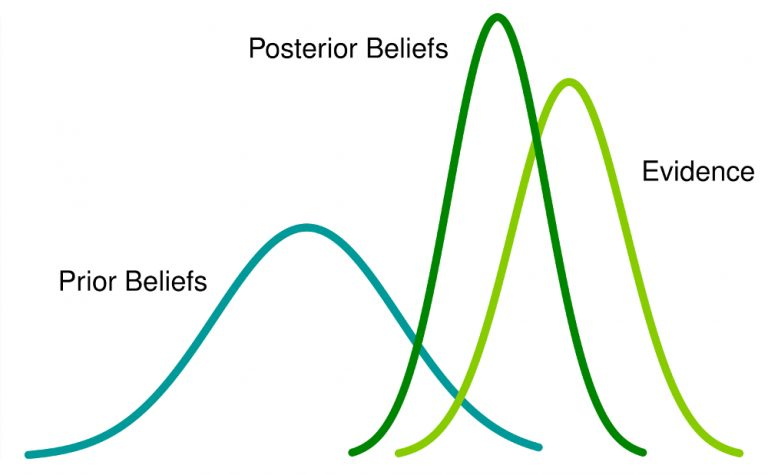
\includegraphics[
  width=15cm,
  height=6cm,
  keepaspectratio,]
{./pics/bayes.jpg}



\end{frame}

%----------------------------------------------------------------------------------------
\begin{frame}
\frametitle{Prediction}

The {\bf prior predictive distribution}: when you haven't seen any data yet:

\[
p(y) = \int p(y \mid \theta) p(\theta) \text{d}\theta
\]
\pause

The {\bf posterior predictive distribution}: when you've seen data 
\begin{align*}
p(\tilde{y} \mid y) &= \int p(\tilde{y}, \theta \mid y) \text{d}\theta \\
&= \int p(\tilde{y} \mid \theta, y) p(\theta \mid y) \text{d}\theta \\
&= \int p(\tilde{y} \mid \theta ) p(\theta \mid y) \text{d}\theta \tag{cond. indep.}
\end{align*}

Both are averages but with different distributions for $\theta$

\end{frame}


%----------------------------------------------------------------------------------------
\begin{frame}
\frametitle{Exchangeability}

Often $y = (y_1, \ldots, y_n)$ are assumed to be {\bf exchangeable}, or

\[
p_{Y_1, \ldots, Y_n}(y_1, \ldots, y_n) = p_{Y_\sigma(1), \ldots, Y_\sigma(n)}(y_1, \ldots, y_n)
\]
where $\sigma$ is any permutation of the indexes.
\pause
\newline

For example, assume $Y_1, Y_2$ are discrete. Then $p(Y_1 = a, Y_2 = b) = p(Y_2 = a, Y_1=b)$.

\end{frame}


%----------------------------------------------------------------------------------------
\begin{frame}
\frametitle{Exchangeability}

The iid condition implies exchangeability:

\begin{align*}
p_{Y_1, \ldots, Y_n}(y_1, \ldots, y_n) &= \prod_{i=1}^n p_{Y_i}(y_i) \tag{indep.} \\
&= \prod_{i=1}^n p_{Y_{\sigma(i)}}(y_i) \tag{ident.} \\
&= p_{Y_{\sigma(1)}, \ldots, Y_{\sigma(n)}}(y_1, \ldots, y_n)
\end{align*}

\end{frame}


%----------------------------------------------------------------------------------------
\begin{frame}
\frametitle{Exchangeability}

However, it isn't the other way around. We will often take $p(y) = \int p(y \mid \theta) p(\theta) \text{d}\theta$

\begin{align*}
p(y) &= p(y_1, \ldots, y_n) \\
&= \int p(y_1, \ldots, y_n \mid \theta) p(\theta) \text{d}\theta \\
&= \int p(y_{\sigma(1)}, \ldots, y_{\sigma(n)} \mid \theta) p(\theta) \text{d}\theta \\
&= p(y_{\sigma(1)}, \ldots, y_{\sigma(n)})
\end{align*}
 but $p(y)$ does not factor

\end{frame}

%----------------------------------------------------------------------------------------
\begin{frame}
\frametitle{LTE and LTV}

Apply the law of total expectation:
\[
\underbrace{E[\theta]}_{\text{prior mean}} = E[\underbrace{E(\theta \mid y)}_{\text{posterior mean}}]
\]
outer expectation on the rhs is taken with respect to $p(y)$.

\end{frame}

%----------------------------------------------------------------------------------------
\begin{frame}
\frametitle{LTE and LTV}

Apply the law of total variance:
\[
\underbrace{var[\theta]}_{\text{prior variance}} = E[\underbrace{var(\theta \mid y)}_{\text{posterior var}}] + \underbrace{var[E(\theta \mid y)]}_{\text{dispersion of post. mean}}
\]
outer expectation on the rhs is taken with respect to $p(y)$.

\end{frame}

%----------------------------------------------------------------------------------------
\begin{frame}
\frametitle{Computation}

We will be using \texttt{R}
\newline


Some bookmarks:
\begin{enumerate}
\item \url{https://github.com/tbrown122387/stat_6440} 
\item \url{http://www.stat.columbia.edu/~gelman/book/}
\item \url{https://github.com/avehtari/BDA_R_demos}
\item \url{http://www.stat.columbia.edu/~gelman/book/data/}
\end{enumerate}



\end{frame}



\end{document} 
